\documentclass{minimal}
\usepackage{fontspec}
\usepackage{tikz}
\usetikzlibrary{calc,angles,quotes,shapes}

\begin{document}

\begin{tikzpicture}[auto]
    \coordinate (o) at (0, 0);
    \coordinate (x) at (3, 0);
    \coordinate (y) at (1, 2);
    \node (xl) at (x) [below] {$x$};
    \node (yl) at (y) [left] {$y$};
    \coordinate (r) at ($ (x) + (y) $);
    \node[inner sep=0pt] (rouel) at (r) [above]
        {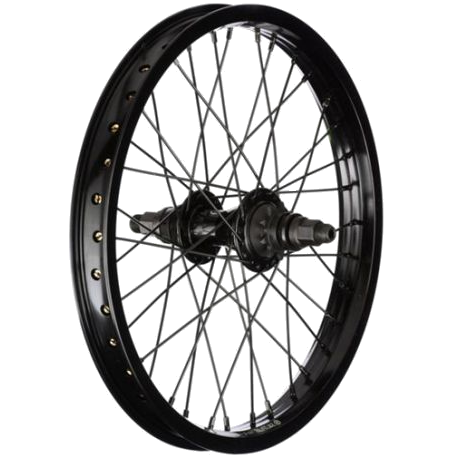
\includegraphics[width=2cm]{roue.png}};
    \draw [->] (o) -- ($ (x) + (x) $);
    \draw [->] (o) -- ($ (y) + (y) $);
    \draw (x) -- (r);
    \draw (y) -- (r);
    \coordinate (t) at (1, 0);
    \draw [->] (t) -- ($ (r) + (r) - (t) $);
    \pic [draw, ->, -latex, "$\theta$", angle radius=30, angle eccentricity=1.3] { angle = x--t--r };
\end{tikzpicture}

\end{document}
